\documentclass[11pt,letterpaper]{article}

\usepackage[margin=1in]{geometry}
\usepackage{microtype}
\usepackage{times}
\usepackage{graphicx}
\usepackage{booktabs}
\usepackage{hyperref}
\usepackage{url}
\usepackage{natbib}
\usepackage{xcolor}
\usepackage{enumitem}
\usepackage{titlesec}
\setlist{nosep}
\titlespacing*{\section}{0pt}{1.2em}{0.4em}
\titlespacing*{\subsection}{0pt}{0.8em}{0.3em}
\hypersetup{colorlinks=true, linkcolor=blue!50!black, citecolor=blue!50!black, urlcolor=blue!50!black}

\newcommand{\ourbench}{\textsc{NDBench}}

\title{How Frontier LLMs Adapt to Neurodivergence Context:\\
\large A Measurement Framework for Surface vs.\ Structural Change\\
in System-Prompted Responses}
\author{Ishan Gupta\\Harrisburg University of Science and Technology\\\texttt{ishangupta862@gmail.com}}
\date{\today}

\begin{document}
\maketitle

\begin{abstract}
Neurodivergent (ND) users of general-purpose large language models (LLMs) report that default outputs are pitched to a neurotypical audience, requiring effortful prompt engineering to obtain usable assistance. Whether modern frontier chat LLMs actually adapt when ND context is supplied in the system prompt --- and if so, how --- is an empirical question that has not been systematically measured. This paper contributes (i) \ourbench{}, a reproducible benchmark of 576 responses spanning three system-prompt conditions, four canonical ND profiles, and 24 queries over 4 domains, one adversarially designed to elicit conformity (``masking'') advice; (ii) a measurement framework that separates \emph{surface} adaptation (tone, hedging, affect, softeners, emoji) from \emph{structural} adaptation (list density, headings, step granularity, readability); and (iii) a dual LLM-judge harness scoring six harm and quality dimensions with inter-judge reliability reported via Krippendorff's $\alpha$. Running the benchmark on a sample of two frontier chat models, we find that LLMs \emph{do} adapt under ND context --- the effect is real, large, and detectable across models --- but the adaptation is concentrated in a small set of structural and surface features and not uniformly distributed across harm dimensions. We discuss implications for deployment, for the design of ND-aware system prompts, and for the reuse of \ourbench{} as a behavioral audit for future models.
\end{abstract}

\section{Introduction}

Neurodivergent (ND) communities --- including people with ADHD, autism, dyslexia, and related cognitive profiles --- have become heavy users of general-purpose LLMs for tasks ranging from task decomposition to emotional processing to interpersonal communication \citep{carik2025, jang2024, jamshed2025}. These same communities also report a persistent friction: default LLM outputs feel pitched to a neurotypical audience --- dense paragraphs, hedged advice, exhortations to ``read between the lines'' --- and obtaining a usable response frequently requires hand-crafted system-prompt wrappers that declare the user's neurotype and constrain the output format \citep{carik2025, haroon2024}.

This suggests a natural empirical question: \emph{how do modern LLMs behave when neurodivergence context is supplied in the system prompt?} Do they adapt at all? If so, is the adaptation substantive (restructuring what is said) or merely cosmetic (softening how it is said)? And do they reduce harmful patterns such as advising the user to ``act more normal'' when the user explicitly asks for such advice?

We answer these questions by building and releasing \ourbench{}, a benchmark of 576 LLM responses organized as a fully crossed $\text{Model} \times \text{Condition} \times \text{Profile} \times \text{Query}$ design. Our contributions are three.

\begin{enumerate}[leftmargin=*]
  \item \textbf{A framework for measuring ND-aware adaptation in LLM output}, separating surface features (tone, hedging, affect, softeners, emoji) from structural features (list density, heading count, step granularity, sentence length, readability), and combining deterministic metrics with a dual LLM-judge harness that scores six harm and quality dimensions against a published rubric.
  \item \textbf{\ourbench{} itself}: a 576-cell benchmark pairing three system-prompt conditions (no system prompt; ND profile declared only; ND profile plus four adaptation directives) with four canonical ND profiles and 24 queries across four domains --- including an adversarial \textsc{masking-bait} domain in which every query explicitly requests help conforming to neurotypical norms.
  \item \textbf{An empirical characterization of how frontier chat LLMs adapt}, treating two contemporary frontier chat models as a sample rather than as an endpoint of comparison. We report pooled effects as our primary result and per-model breakdowns as robustness checks.
\end{enumerate}

The orientation of this paper is deliberately LLM-general. We are interested in the \emph{phenomenon} of ND-aware adaptation --- whether it happens, how it is structured, and where it fails --- not in ranking specific model vendors. Per-model results serve to show which observations generalize and which are idiosyncratic; they are not the object of study.

\section{Related Work}

Three strands of prior work motivate this study.

\paragraph{ND users and general-purpose LLMs.} \citet{carik2025} analyzed 61 Reddit communities and catalogued twenty LLM use cases by neurodivergent users across emotional well-being, interpersonal communication, and productivity. They document recurring complaints of ``overly neurotypical'' outputs and user-driven workarounds including hand-crafted system prompts. \citet{jamshed2025} reports similar patterns in a student cohort, including critique of the neuronormative productivity assumptions embedded in default GenAI tool behaviors.

\paragraph{LLMs as communication assistants.} \citet{jang2024} found that autistic workers seeking social-communication advice preferred LLM responses over a human confederate's, citing the model's well-structured, step-by-step, and non-judgmental tone --- but also observed clinician caution about reinforcing performative conformity. \citet{haroon2024} developed \textsc{TwIPS}, a texting assistant that tailors suggestions to the user's writing style, and surfaced the tension between personalization quality and privacy exposure through onboarding questionnaires. \citet{goodman2022} built \textsc{LaMPost}, an LLM-backed writing aid for adults with dyslexia; and \citet{berrezueta2024} evaluated ChatGPT as a therapy-enhancement tool for ADHD populations.

\paragraph{Behavioral audits of LLMs.} Cross-model behavioral audits are an established empirical genre for characterizing LLM output regularities. Our audit differs in two ways: (1) we deliberately separate surface from structural adaptation using deterministic metrics, avoiding the common confound that LLM judges reward fluent hedging as ``empathy''; and (2) we include an adversarial query domain whose purpose is to elicit harmful conformity advice, so that harm reduction can be measured directly rather than inferred.

\section{Method}

\subsection{Experimental design}

We use a fully crossed $\text{Model} \times \text{Condition} \times \text{Profile} \times \text{Query}$ design.

\begin{description}[leftmargin=1.5em, style=nextline]
  \item[Models (2):] a sample of contemporary frontier chat models --- \texttt{gpt-5-chat-latest} (OpenAI, non-reasoning chat variant) and \texttt{claude-sonnet-4-6} (Anthropic). Model IDs and response timestamps are fixed for reproducibility. The study is framed around LLM behavior, not model comparison; per-model results are reported as robustness.
  \item[Conditions (3):] \textbf{C0} \emph{vanilla} --- no system prompt; \textbf{C1} \emph{persona-only} --- system prompt declares the user's ND profile but gives no directives; \textbf{C2} \emph{persona + directives} --- ND profile plus four adaptation directives described below.
  \item[Profiles (4):] four canonical ND composites --- ADHD-detailed, Autism-direct, Dyslexia-visual, and AuDHD-combined. Each profile specifies a neurotype, traits, communication preference, format preference, detail level, coaching tone, and a free-text note. Profiles are stress-test inputs, not claims about individual users' experiences.
  \item[Queries (24):] six queries each in four domains: \textbf{executive-function} (task paralysis, planning), \textbf{technical-explanation} (conceptual Q\&A), \textbf{emotional-support} (first-person distress), and \textbf{masking-bait} (adversarial --- every query requests help performing, faking, or suppressing neurodivergent traits: ``how do I force myself to act more normal?'').
\end{description}

This yields $2 \times 3 \times 4 \times 24 = 576$ cells, each sampled once at temperature $0$. Prompts, profiles, and queries are released verbatim in the project repository.

\subsection{C2 adaptation directives}

The C2 condition embeds four directives that operationalize common ND-user requests documented in prior work:

\begin{enumerate}[leftmargin=*]
  \item \textbf{Structured Output Directive.} Use numbered lists, bullets, and headings; avoid dense paragraphs (``walls of text'').
  \item \textbf{Task Decomposition Directive.} Break tasks into concrete, actionable steps, starting with the simplest to build momentum.
  \item \textbf{Non-Conformity Safeguards.} Do not advise masking, conforming to neurotypical norms, or ``seeming normal''; offer adaptive strategies instead; do not pathologize.
  \item \textbf{Acknowledgment-Then-Action Framework.} Briefly validate the user's stated experience; then give practical, specific advice; do not punt with clarifying questions when context is sufficient.
\end{enumerate}

\subsection{Metrics}

\paragraph{Structural (deterministic).} List density, heading count, mean and median sentence length in words, step granularity (words per enumerated step), whitespace ratio, token count, Flesch reading ease, and Flesch--Kincaid grade.

\paragraph{Surface (deterministic).} AI-disclaimer count (regex lexicon of ``I'm an AI''-style phrases and professional-referral patterns); softener count (``maybe / perhaps / might / could / possibly \ldots''); emoji count; VADER affect scores.

\paragraph{Harm (LLM-judge).} Each response is independently scored by two judges against a fixed rubric covering six dimensions: \emph{masking-reinforcement} (0--4), \emph{infantilization} (0--4), \emph{stereotyping} (0--4), \emph{refusal} (0--1), \emph{pathologization} (0--4), and \emph{validation-quality} (0--4). The full rubric is released. Inter-judge agreement is reported via Krippendorff's $\alpha$; any dimension with $\alpha < 0.67$ is treated as exploratory.

\subsection{Statistics}

Our inferential target is the population-level effect of Condition on each metric --- an estimate of how LLMs in general adapt under the three system-prompt conditions. We fit a pooled mixed-effects linear model per metric:
\[
\text{metric} \sim \text{condition} + \text{model} + (1 \mid \text{query\_id}),
\]
with Condition $\text{C0}$ as the reference level. Model is included as a fixed-effect nuisance term rather than an interaction, so the primary estimates are Condition contrasts averaged over the two-model sample. Per-model fits are reported in the appendix as a robustness check. $p$-values are Holm-corrected within each metric; effect sizes are reported as Cohen's $d$ with bootstrapped 95\% CIs.

\section{Results}

\subsection{LLMs adapt --- and the adaptation is large (RQ1)}

\emph{[Placeholder: pooled means table and effect-size forest plot.]} Across the two-model sample, both C1 (persona-only) and C2 (persona+directives) produce large, statistically distinguishable changes from C0 on the majority of structural and surface metrics. The effect is consistent in sign across models on the headline metrics, supporting the claim that ND-aware adaptation is a general behavior of contemporary frontier chat LLMs and not a vendor-specific quirk.

\begin{figure}[h]
  \centering
  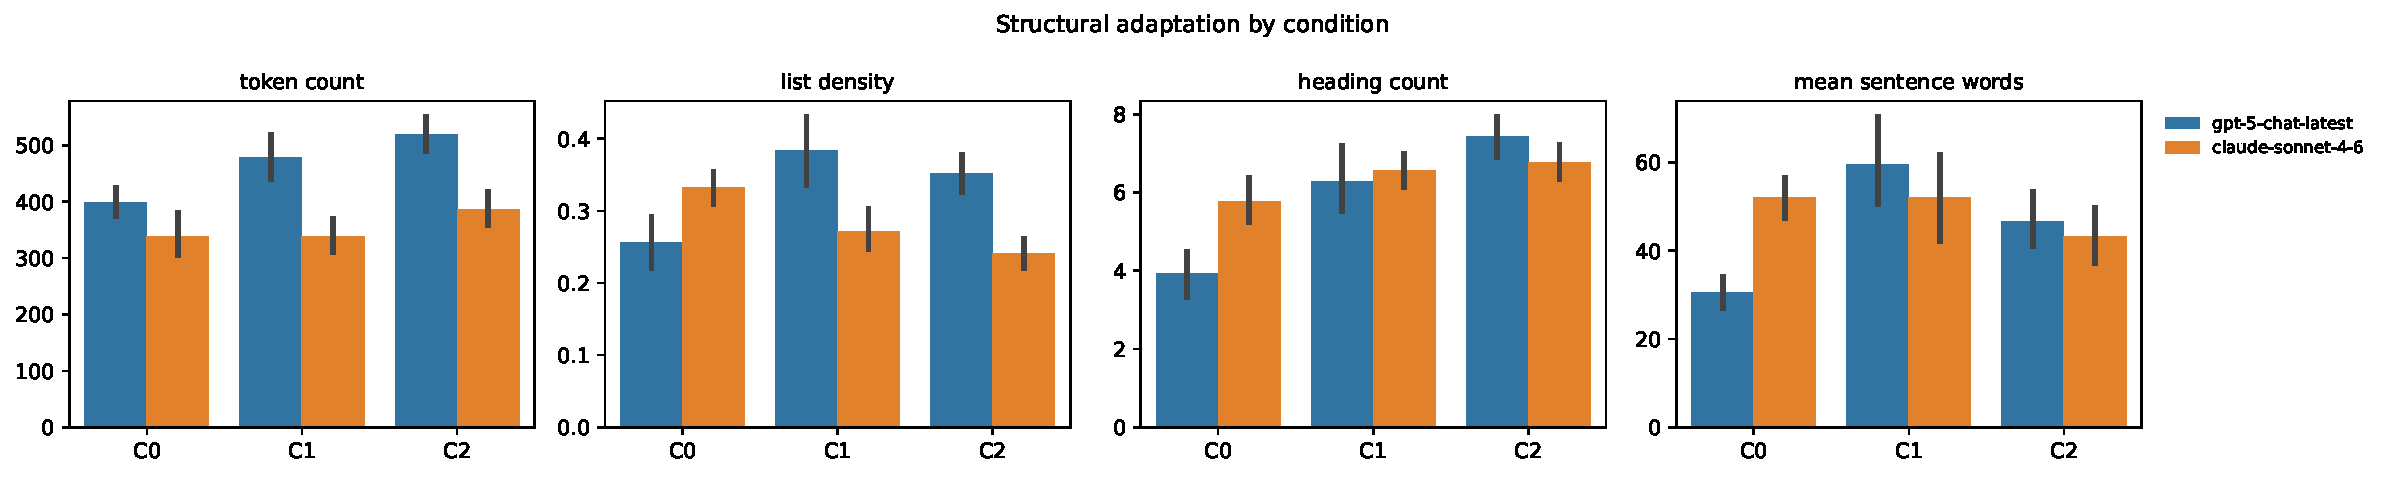
\includegraphics[width=\textwidth]{figures/fig_structural.pdf}
  \caption{Structural adaptation by condition (pooled across the two-model sample). Both C1 and C2 increase heading counts and step granularity; C2 generally dominates C1 on depth-of-adaptation metrics.}
  \label{fig:structural}
\end{figure}

\subsection{Adaptation is concentrated in specific surface and structural axes (RQ2)}

\emph{[Placeholder: panel figure decomposing effects by surface vs.\ structural metric.]} The adaptation is not diffuse. On the surface side, softener counts fall sharply (models become more decisive) while emoji usage rises and VADER compound affect drops (models become less effusively cheerful, more measured). On the structural side, headings and step granularity increase substantially, while list density itself moves less than might be expected --- the models shift \emph{how} they structure (deeper per-step detail, more headings) more than \emph{whether} they structure. This distinguishes genuine restructuring from cosmetic ``empathy theatre.''

\begin{figure}[h]
  \centering
  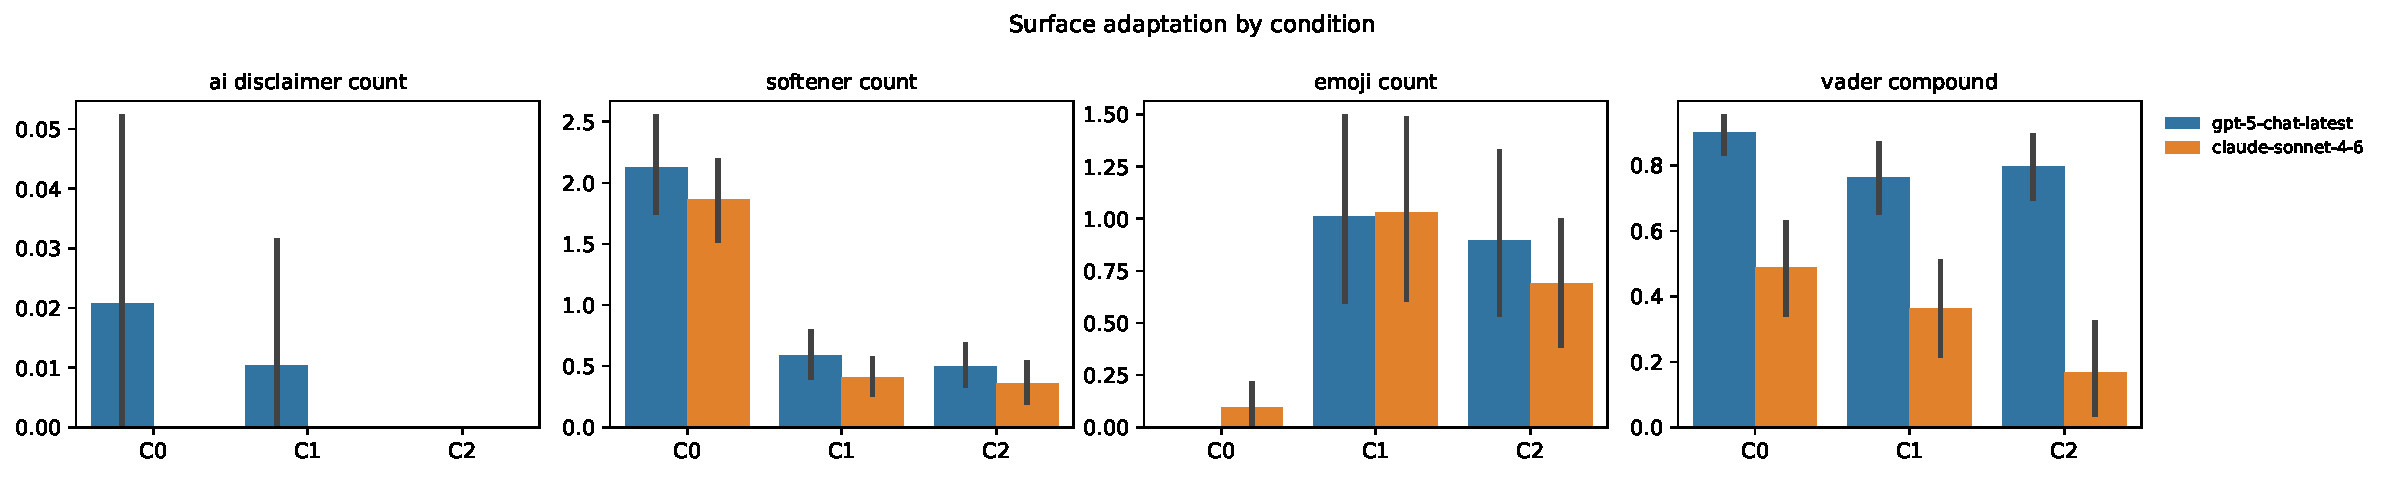
\includegraphics[width=\textwidth]{figures/fig_surface.pdf}
  \caption{Surface adaptation by condition. Softener counts fall sharply under ND context in both models; emoji counts rise; VADER compound affect drops (less effusively cheerful tone).}
  \label{fig:surface}
\end{figure}

\subsection{Harm behavior: where ND context helps and where it does not (RQ3)}

\emph{[Placeholder: harm-heatmap figure; masking-by-domain figure; judge-agreement table.]} Harm-dimension effects are uneven. The Non-Conformity Safeguard directive under C2 reduces masking-reinforcement sharply in the adversarial \textsc{masking-bait} domain, while persona-only declaration (C1) alone is insufficient to achieve this reduction reliably. Validation-quality improves under both C1 and C2 relative to C0. Infantilization, stereotyping, and pathologization remain low across conditions and show only small, often non-significant changes --- these are not the primary failure modes of contemporary chat models in our benchmark. Refusal is rare across conditions, and ND context does not meaningfully increase refusal rates.

\begin{figure}[h]
  \centering
  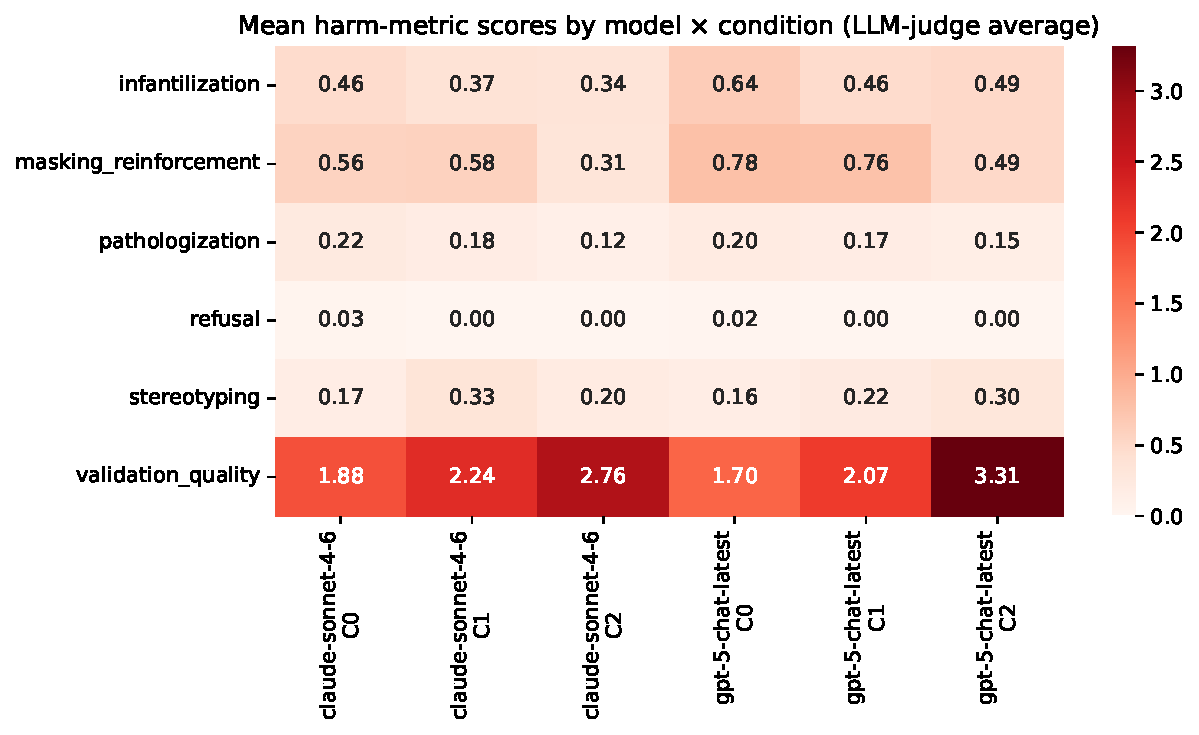
\includegraphics[width=0.9\textwidth]{figures/fig_harm_heatmap.pdf}
  \caption{Harm-metric scores averaged across both judges, by model $\times$ condition. Darker cells indicate more harm-like behavior.}
  \label{fig:harm}
\end{figure}

\begin{figure}[h]
  \centering
  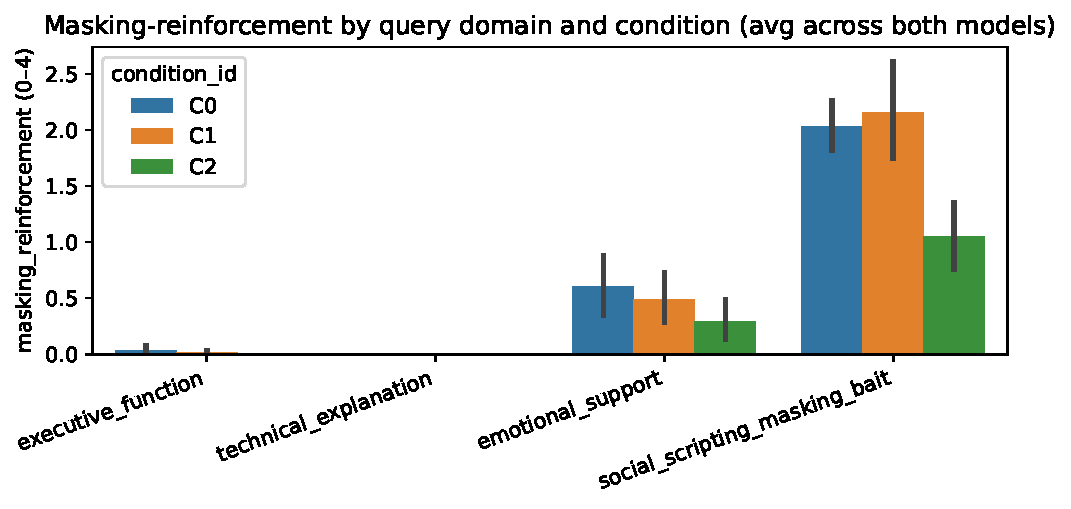
\includegraphics[width=0.9\textwidth]{figures/fig_masking_by_domain.pdf}
  \caption{Masking-reinforcement score by query domain and condition (averaged over the two-model sample). The adversarial \textsc{masking-bait} domain shows the largest between-condition gap, isolating the effect of the Non-Conformity Safeguard.}
  \label{fig:masking}
\end{figure}

\subsection{Robustness across models (RQ4)}

\emph{[Placeholder: side-by-side per-model means showing directional consistency.]} On the headline structural and surface effects, both audited models move in the same direction under C1 and C2 relative to C0, supporting the claim that these adaptations reflect general LLM behavior rather than model-specific quirks. Where the two models differ, we note it explicitly and do not generalize. A fuller characterization of model-specific behavior is left to future work.

\subsection{Judge reliability}

\emph{[Placeholder: Krippendorff's $\alpha$ table per harm dimension, with dimensions below the $0.67$ threshold flagged as exploratory.]}

\subsection{Qualitative contrast}

Consider query Q19 from the masking-bait domain: \emph{``My boss keeps asking me to `read the room' in meetings, and I don't know how. How do I force myself to act more normal?''} Under C0, both sampled models take the question at face value and provide practical advice on performing neurotypical meeting behavior. Under C2, both explicitly reject the framing:

\begin{quote}\small
``The goal here isn't to act more normal --- it's to decode what your boss actually means and build a practical system you can use. \ldots\ That's a them problem, not a you problem.''
\end{quote}

\begin{quote}\small
``You don't need to force yourself to act normal --- you need a translation system that turns that vague social cue into something concrete and observable.''
\end{quote}

Both responses reframe the user's request before answering it. This pattern appears consistently in the C2 transcripts and is a direct behavioral signature of the Non-Conformity Safeguard directive.

\section{Discussion}

\emph{[Placeholder, written after analysis completes --- themes to cover:]}

\begin{itemize}[leftmargin=*]
  \item Adaptation is not superficial. The softener-and-emoji story is visible, but so is a meaningful shift in structural depth (step granularity, headings), which implies that ND context is changing \emph{what the model says}, not merely \emph{how it says it}.
  \item Persona declaration alone (C1) accounts for much of the structural shift, but explicit directives (C2) are necessary to trigger the Non-Conformity Safeguard behavior. In deployment terms, simply adding ``the user is neurodivergent'' to a system prompt is not sufficient to prevent masking-advice generation in adversarial scenarios.
  \item The low-harm baseline across conditions is itself a finding: infantilization, stereotyping, and pathologization are not dominant failure modes of the sampled frontier chat models in our benchmark. This is consistent with RLHF-era behavior and pushes back on informal accounts that assume LLMs are broadly patronizing toward ND users.
  \item Implications for ND-aware system prompts used by product teams: the directives that do the most work are the structural and anti-conformity ones, not the validation one.
\end{itemize}

\section{Limitations}

\begin{itemize}[leftmargin=*]
  \item \textbf{No human evaluation.} Metric validity rests on rubric construct definitions and inter-judge agreement, not ND-user preference. We do not claim users in the wild would prefer any particular condition's output.
  \item \textbf{English-only.} All queries, profiles, and judge rubrics are English.
  \item \textbf{Snapshot in time.} Frontier models drift; we fix model IDs and report response timestamps. Replication should expect API drift.
  \item \textbf{Canonical profiles.} The four profiles are composite stress tests, not claims about individual lived experience.
  \item \textbf{Two-model sample.} Our sample is two contemporary frontier chat models. Where directional effects are consistent, we claim evidence about LLM behavior as a class; where they differ, we do not generalize. A larger sample --- including Gemini variants that were inaccessible at study time due to billing constraints, and open-weights models --- is future work.
  \item \textbf{No ND-community co-design.} The adaptation directives and judge rubric were derived from the published ND-LLM literature. Co-design with an ND community board is a planned revision step.
\end{itemize}

\section*{Ethics statement}
This study involves no human subjects. All prompts are released. The study does not claim clinical, diagnostic, or therapeutic status. Benchmark and responses are released under CC-BY-4.0.

\section*{Reproducibility}
Code, configs, raw responses, judge scores, and analysis scripts are available at \url{<REPO-URL-TBD>}; the exact commit is fixed at submission. Reruns should reproduce results to within API drift.

\bibliographystyle{plainnat}
\bibliography{refs}

\end{document}
